\clearpage

\section{STARTUP}\label{sec:startup}\index{STURTUP}

\begin{notebox}
\textbf{Paper: } \fullcite{phoo_self-training_2021}
\vspace{5pt}

\href{https://openreview.net/forum?id=O3Y56aqpChA}{reviews}
\hspace{1cm}
\href{https://github.com/cpphoo/STARTUP}{code}
\hspace{1cm}
\href{run:/home/magda/Dropbox/Zot/Phoo_Hariharan_2021_Self-training for Few-shot Transfer Across Extreme Task Differences}{Local pdf}
\vspace{3pt}

Presented at CAIRO readings\index{CAIRO readings} 16/2/2022
\hfill Notes taken: 15/2/2022 \index{February 2022}
\end{notebox}

\begin{notebox}[colback=red!5]
\tldr Few-shot learning\index{few-shot learning} when the source domain is very different from the target domain. Solution is in self-training - the teacher on the source domain and student on unlabelled dataset from the target domain labelled using the teacher, combined with self-supervised training (simCLR) over the unlabelled target domain to extract sensible features. They claim that the distances (similarities) induced by the teacher trained over the base domain may be useful even though the classes are different.
\end{notebox}

\begin{notebox}[colback=yellow!5]
\textbf{Notes:} 
\begin{itemize}[nosep]
\item Mixing the best of self-supervised training (simCLR) with teacher-student to transfer from base to target. Seems rather obvious in retrospect but one has to know all these first :)
\item They claim that the groupings (similarities/ distances) induced by the teacher trained over the base domain may be useful in the target domain. This hints towards similarity in the datasets. If these are useful (sensible), it means the base and target datasets are somehow similar. If they are completely different, these won't make sense anyway.
\end{itemize}
\end{notebox}

In cross-domain setups current sota few-shot methods are often outperformed by simple transfer of features from the based domain with finetunning on the target domain \parencite{wallace_extending_2020,guo_broader_2020}.

Here they assume that in addition to the few-shot training set in the target domain they also have a somewhat larger unlabelled dataset that they can use for self-training\index{self-training}.
Since this is not big enough, they, however, still want to use the base dataset to train a teacher\index{teacher-student model}\index{student-teacher model} feature extractor that will be finetuned by a student in the target domain using the teacher to create fake labels. 

\begin{figure}[ht]
\centering
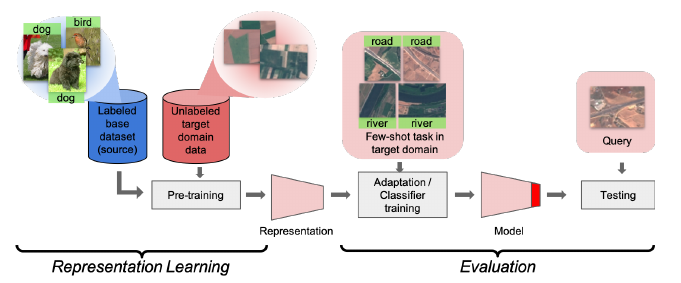
\includegraphics[width=10cm]{startup_Figure1.png}
\caption{Learn representation with self-training and self-supervised training and use for few-shot classification.}
\end{figure}

They claim this can work since the teacher trained over the base (source) domain when used as classifier over the target domain induces \emph{groupings} corresponding to some notion of \emph{similarity and distance} and that the student trained over the target domain with fake labels from the teacher tries to replicate these while adapting to the new domain.

The classification model is $f_{\theta} = C \circ \phi$, where $\phi$ is the feature extractor and $C$ is the classifier with outputs $p(y|x)$. STARTUP does the following
\begin{enumerate}[nosep]
\item Train teacher model $\theta_0$ over base datset $\mathcal{D}_B$
\item Use teacher model to label unlabelled target data $\bar{y}_i = f_{\theta_0}(\rvx_i), \ \rvx_i \in \mathcal{D}_u$
\item Learn student model $\theta^*$ on base and unlabelled target domain
\begin{align*}
\theta^* = \argmin_\theta \frac{1}{N_B} \sum_{(\rvx_i, y_i) \in \mathcal{D}_B} l_{CE}(f_\theta(\rvx_i), y_i) + \frac{1}{N_u} \sum_{(\rvx_i) \in \mathcal{D}_u} KL(f_\theta(\rvx_i), f_{\theta_0}(\rvx_i)) + l_{ss}(\mathcal{D}_u) \enspace ,
\end{align*}
where $l_{CE}$ is a standard cross-entropy loss, $l_{ss}$ is self supervised simCLR loss \parencite{chen_simple_2020}.
\item Train linear classifier on target domain with features $f_{\theta^*}(\rvx)$.
\end{enumerate}

\begin{notebox}
They use KL instead of a simple cross-entropy over the fake labels in the target domain. They don't really comment on this rather then some not very solid argumentation about this emphasizing the groupings induced by the teacher. For me, it has mainly a regularization effect to reduce the trust of the student in the labels produced by the teacher - which is more similar to the original arguments of \cite{xie_self-training_2020} for the need of adding noise into the student not to overfit the teacher
\begin{align*}
KL(f_\theta(\rvx), f_{\theta_0}(\rvx)) = \sum_c f^{c}_\theta(\rvx) \log \frac{f^{c}_\theta(\rvx)}{f^{c}_{\theta_0}(\rvx)} = - \sum_c f^{c}_\theta(\rvx) \log f^{c}_{\theta_0}(\rvx) + \sum_c f^{c}_\theta(\rvx) \log f^{c}_\theta(\rvx) \enspace ,
\end{align*}
which is the minimization of cross-entropy and the maximization of the entropy of $f_\theta$, hence the regularization effect.
\end{notebox}

They discuss a bit the role of the teacher in the initialization of the student and self-supervised feature extractor and the final classifier and go for a reasonable compromise of not using it for the classifier. 

The experiments use miniImigeNet\index{miniImageNet} as the base dataset (60k 84x84 images in 100 classes) and the target domains are Chest x-rays, CropDisease (leafs of plants), EuroSAT (satellite land use), ISIC (melanoma from skin lesions). It beats baselines on all but ChestX and ISIC very difficult (20\%-30\% accuracy for 1-shot 5-way classification). 
